% Chronos-Hydrodynamics — Paper 2 (EM–GPE Casimir derivation)
% Compiler: pdfLaTeX + Biber
% Upload with references.bib and figures/ (see README.md)

\documentclass[11pt,a4paper]{article}

\usepackage[margin=1in]{geometry}
\usepackage{amsmath,amssymb,amsfonts}
\usepackage{graphicx}
\usepackage{booktabs}
\usepackage{enumitem}
\usepackage{xcolor}
\usepackage{hyperref}
\usepackage{siunitx}
\usepackage[backend=biber,style=numeric,sorting=none,maxbibnames=99]{biblatex}
\usepackage{placeins}  % \FloatBarrier — keep figures from drifting past section breaks

% Loosen float placement slightly so figures stay nearer their source
\renewcommand{\topfraction}{0.9}
\renewcommand{\bottomfraction}{0.85}
\renewcommand{\textfraction}{0.08}
\renewcommand{\floatpagefraction}{0.75}

\graphicspath{{figures/}}

\addbibresource{references.bib}

\hypersetup{
  colorlinks=true,
  linkcolor=blue!60!black,
  citecolor=blue!60!black,
  urlcolor=blue!60!black
}

\title{%
  Deriving the Gated Casimir Ripple from Gross--Pitaevskii Boundary States\\
  and Electromagnetic Coupling in Chronos-Hydrodynamics%
}
\author{%
  George McNally\\[0.25em]
  \small Independent Researcher\\[0.15em]
  \small \href{mailto:george@web-essentials.ie}{george@web-essentials.ie}%
}
\date{Draft --- \today}

\begin{document}

\maketitle

\begin{abstract}
Paper~1 of Chronos-Hydrodynamics (CH) parameterizes a gated oscillatory correction to the normalized Casimir force,
$F(d)/F_{\mathrm{Cas}}(d) = 1 + \alpha_{\mathrm{eff}}(k)\cos(2\pi d/a_{\mathrm{vac}} + \phi)$ with
$\alpha_{\mathrm{eff}} = \alpha_{\max}\chi(|\nabla\rho|)$, and provides a pre-registered laboratory protocol
( Prediction~\#7) to test flat vs threshold turn-on in $\alpha(k)$.
This paper derives---or perturbatively motivates---that ansatz by coupling electromagnetic cavity modes to
Gross--Pitaevskii boundary profiles $\rho(z)$ and the gradient gate $\chi$ computed in Paper~1.
We import $\chi_{\mathrm{bulk}}(d)$ and $\chi_{\mathrm{wall}}(R)$ from the existing GPE pipeline, specify an
EM--vacuum coupling $\delta\varepsilon(\rho,\chi)$, and compute $\delta F(d)$ from a mode sum.
Minimum success: $\alpha_{\mathrm{eff}} \propto \chi_{\mathrm{bulk}}(d)$ with QFT recovery as $\chi \to 0$.
Full success: predicted $a_{\mathrm{vac}}(\xi)$ and $\alpha_{\max}(\xi,\rho_{\mathrm{in}})$ with fewer free parameters than Paper~1.
At $\xi=50$\,nm we find corr($\delta F/F_{\mathrm{Cas}},\chi_{\mathrm{bulk}})\approx 0.94$, preferred grain $\kappa\approx 0.02$ ($\alpha_{\max}\approx 0.2\%$),
staged healing $a^*/(2\pi\xi)\approx 0.95$, and multiplicative $F/F_{\mathrm{Cas}}$ preferred over additive ($\Delta\chi^2\approx 141$).
\end{abstract}

\section{Introduction}
\label{sec:intro}

\subsection{Relation to Paper~1}

CH \cite{CHPaper1} states that Eq.~\eqref{eq:casimir-ripple} is \textbf{parameterized}, not derived from the GPE.
The falsifiable claim of that manuscript is Prediction~\#7: threshold vs flat behavior of extracted ripple amplitude $\alpha(k)$
vs laboratory knob $k$, with a mandatory flat control channel.
\textbf{This paper does not replace that protocol.} It addresses Prediction~\#3 and the open problem of a
first-principles EM--GPE derivation of the Casimir ripple.
Paper~1 documents grain-scale $\alpha_G^{\mathrm{hydro,ref}}$, exterior Newton matching (including oblate 2D rays), and a variational $\mathcal{L}_{\mathrm{int,grav}} \Rightarrow \alpha_G$ route parallel to $\kappa$ here~\cite{CHPaper1}; full dynamical $S_M$ remains Layer~2 identification in that manuscript.

Paper~1 assumed
\begin{equation}
  \frac{F(d)}{F_{\mathrm{Cas}}(d)} = 1 + \alpha_{\mathrm{eff}}(k)\,
  \cos\!\left(\frac{2\pi d}{a_{\mathrm{vac}}} + \phi\right),
  \qquad
  \alpha_{\mathrm{eff}} = \alpha_{\max}\,\chi(|\nabla\rho|).
  \label{eq:casimir-ripple}
\end{equation}

\subsection{What we derive vs assume}

\begin{table}[htbp]
  \centering
  \small
  \caption{Three parts of the Casimir ripple ansatz (Paper~1 Eq.~\ref{eq:casimir-ripple}).}
  \label{tab:three-parts}
  \begin{tabular}{@{}lll@{}}
    \toprule
    Part & Content & Paper~2 target \\
    \midrule
    A & $\cos(2\pi d/a_{\mathrm{vac}})$ shape and period & Derive (Route~2 + mode sum) \\
    B & $\alpha_{\mathrm{eff}} = \alpha_{\max}\chi$ & Derive (EM coupling) \\
    C & Probe loci $\chi_{\mathrm{bulk}}$, $\chi_{\mathrm{wall}}$ & Import from Paper~1 \\
    \bottomrule
  \end{tabular}
\end{table}

\section{Layer 1 recap: GPE boundary profiles}
\label{sec:layer1}

Paper~1 solves the stationary 1D GPE between perfect-conductor plates ($\psi = 0$ at walls),
exports $\rho(z)$, $|\nabla\rho|$, and the gradient gate $\chi(|\nabla\rho|)$ vs gap $d$.
At $\xi = 50$\,nm, $\chi_{\mathrm{bulk}}(d)$ peaks near $d \sim 80$--100\,nm and falls toward zero
at large $d$ (QFT recovery). Scripts: \texttt{ch\_gpe\_casimir\_gap.py},
\texttt{ch\_paper2\_gpe\_export.py}. Part~C of Eq.~\eqref{eq:casimir-ripple} is \textbf{imported}, not re-derived here.

\section{EM--GPE coupling}
\label{sec:coupling}

Coupling C1 (locked for Phase 1):
\begin{equation}
  \frac{\varepsilon(z)}{\varepsilon_0}
  = 1 + \kappa\,\chi_{\mathrm{bulk}}(d)\left(1 - \frac{\rho(z)}{\rho_{\mathrm{in}}}\right),
  \qquad \kappa \ll 1.
  \label{eq:coupling-c1}
\end{equation}
Inputs $\rho(z)$, $\chi_{\mathrm{bulk}}(d)$ are exported from the Paper~1 GPE pipeline
(\texttt{ch\_gpe\_casimir\_gap.py}, \texttt{ch\_paper2\_gpe\_export.py}).
See \texttt{docs/paper-2/coupling-spec.md}.

\section{Minimal derivation: gated amplitude}
\label{sec:minimal}

\subsection{Perturbative mode sum}

Perfect conductors at $z=0,d$; TE modes $\psi_n \propto \sin(n\pi z/d)$.
For small static $\delta\varepsilon(z) = \varepsilon(z)/\varepsilon_0 - 1$,
\begin{equation}
  \frac{\delta\omega_n}{\omega_n^{(0)}}
  \approx \int_0^1 \delta(u)\,\sin^2(n\pi u)\,du,
  \qquad u = z/d.
\end{equation}
The leading UV-finite force response uses $n^2$-weighted mode shifts (TE+TM factor~2):
\begin{equation}
  \frac{\delta F}{F_{\mathrm{Cas}}}
  \approx \frac{\sum_{n=1}^{N} n^2\,(\delta\omega_n/\omega_n)}{\sum_{n=1}^{N} n^2}.
  \label{eq:mode-sum}
\end{equation}
Implemented in \texttt{ch\_casimir\_mode\_sum.py}; driver \texttt{ch\_casimir\_em\_coupling.py}.

\subsection{Phase 1 results (Thomas--Fermi \texorpdfstring{$\rho$}{rho}, no lattice)}

At $\xi = 50$\,nm, $\kappa = 0.12$, $n_{\max}=800$:
\begin{itemize}[nosep]
  \item corr($\delta F/F_{\mathrm{Cas}}$, $\chi_{\mathrm{bulk}}$) $\approx 0.94$ (mode sum) vs $0.87$ (toy integral).
  \item peak $|\delta F/F_{\mathrm{Cas}}| \approx 1.8\%$.
  \item $\chi \to 0 \Rightarrow \delta F \to 0$ (QFT recovery).
\end{itemize}
\textbf{Part B (gating):} the EM correction tracks $\chi_{\mathrm{bulk}}(d)$; amplitude is not yet predicted from first principles ($\kappa$ is input).
Figure~\ref{fig:em-gating} plots the mode-sum and toy integral against gap and $\chi_{\mathrm{bulk}}$.

\begin{figure}[htbp]
  \centering
  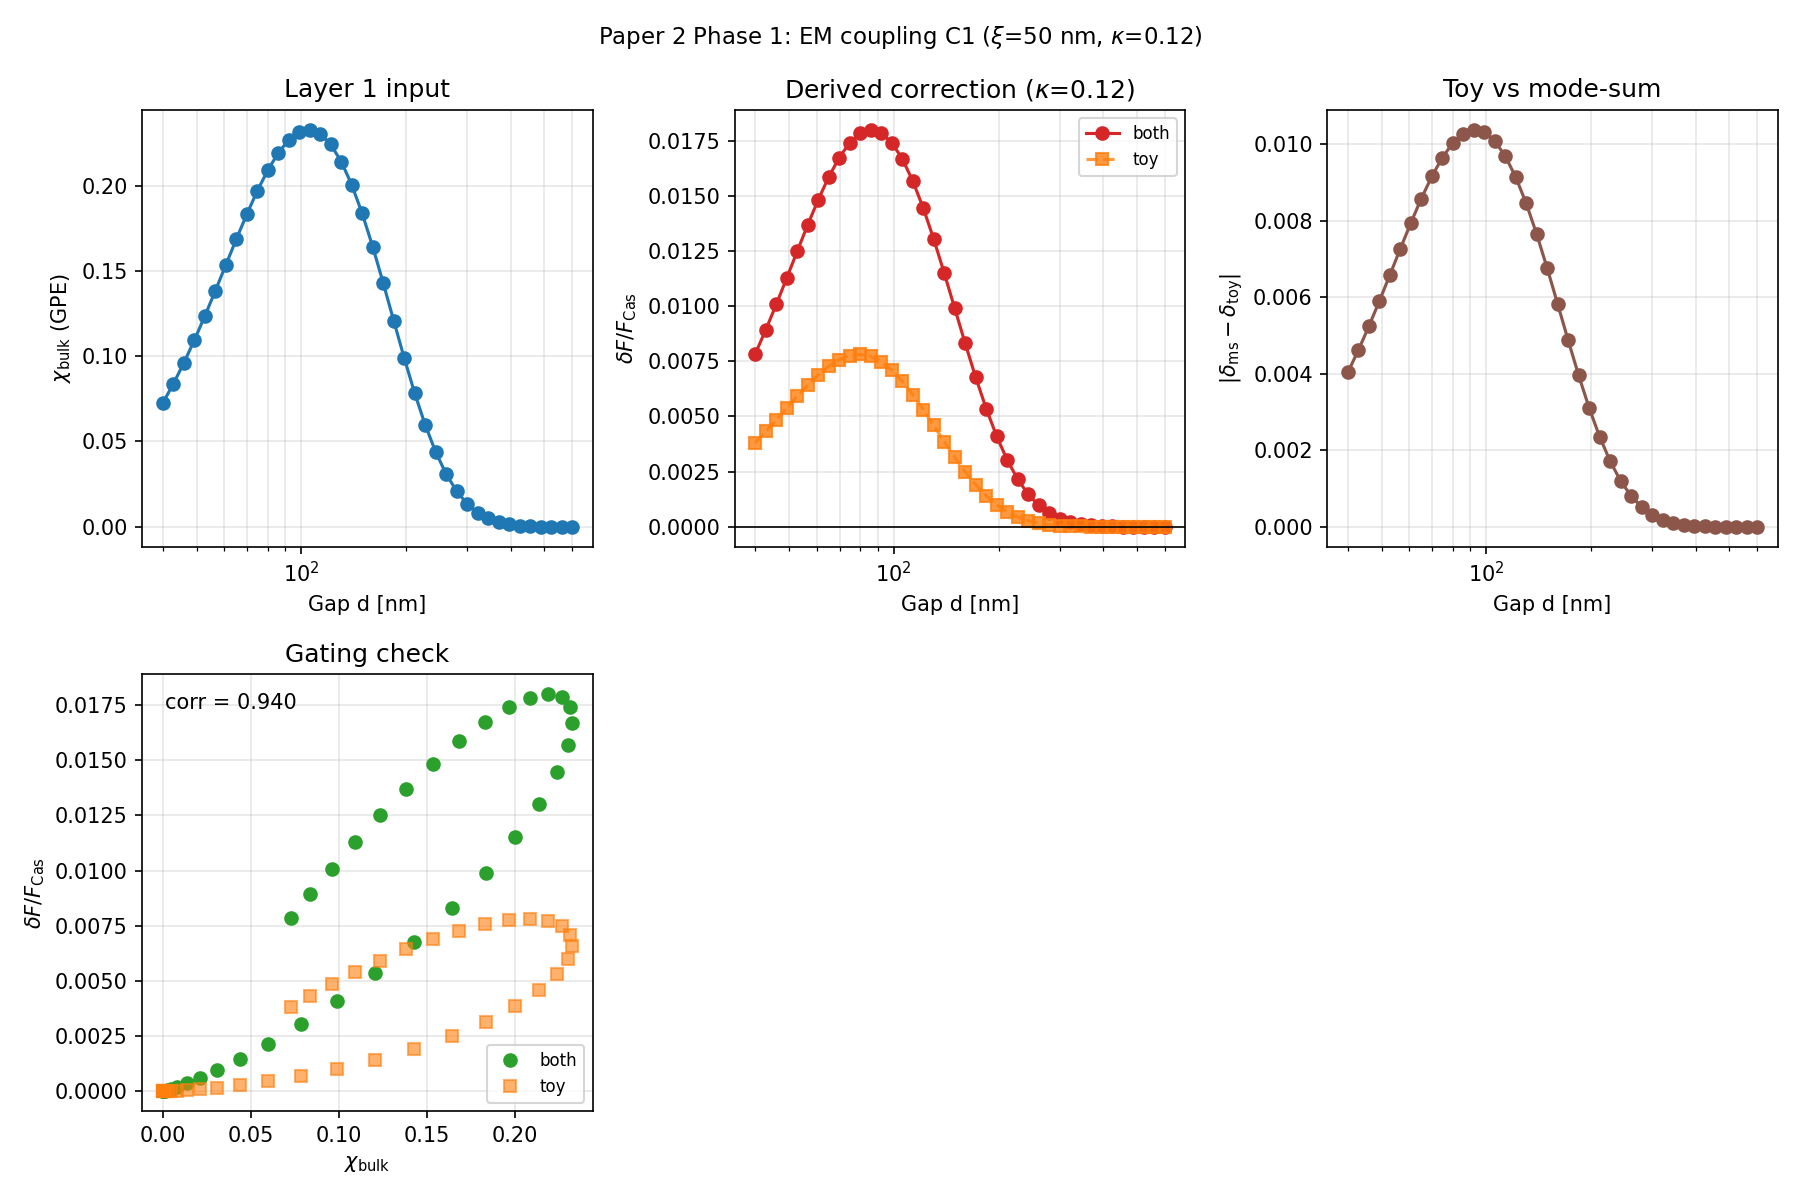
\includegraphics[width=0.92\linewidth]{em_coupling_xi50nm_kappa0p12_both.png}
  \caption{Phase~1b: derived $\delta F/F_{\mathrm{Cas}}$ vs gap and vs $\chi_{\mathrm{bulk}}$ at $\xi=50$\,nm, $\kappa=0.12$ (toy vs mode sum).}
  \label{fig:em-gating}
\end{figure}
\FloatBarrier

\section{Period from vacuum structure}
\label{sec:period}

\subsection{Periodic supersolid ansatz (Phase 2)}

Hybrid profile in the cavity:
\begin{equation}
  \frac{\rho(z)}{\rho_{\mathrm{in}}}
  = \tanh(\hat z)\tanh(\hat d - \hat z)\,
  \bigl[1 + \eta\cos(2\pi z/a_{\mathrm{vac}})\bigr],
  \qquad \hat z = z/\xi.
\end{equation}
Walls suppress modulation where $\rho \to 0$.
Script: \texttt{ch\_casimir\_supersolid\_period.py}.

\subsection{Period calibration}

Direct periodic dielectric test (isolates Part~A):
$\delta\varepsilon/\varepsilon_0 = \kappa\chi\eta\cos(2\pi z/a_{\mathrm{vac}})$ with $\chi=1$.
At imposed $a_{\mathrm{vac}} = 2\pi\xi$ ($\xi=50$\,nm):
fitted $a_{\mathrm{fit}}/a_{\mathrm{imposed}} \approx 1.05$.
\textbf{The mode sum reproduces the Paper~1 cosine period} when a periodic $\varepsilon(z)$ is fed in.

With the full hybrid profile and GPE $\chi_{\mathrm{bulk}}(d)$ envelope, a \textbf{joint fit}
\begin{equation*}
  \delta F/F_{\mathrm{Cas}} \approx \chi_{\mathrm{bulk}}\,\alpha\cos(2\pi d/a + \phi)
\end{equation*}
on $d \lesssim 550$\,nm gives $a_{\mathrm{joint}}/a_{\mathrm{imposed}} \approx 1.2$ at $\eta=0.08$
(vs naive cosine fit $\approx 1.9$ without $\chi$ unfolding).
Figure~\ref{fig:period-cal} shows the periodic dielectric calibration at imposed $a_{\mathrm{vac}} = 2\pi\xi$.

\begin{figure}[htbp]
  \centering
  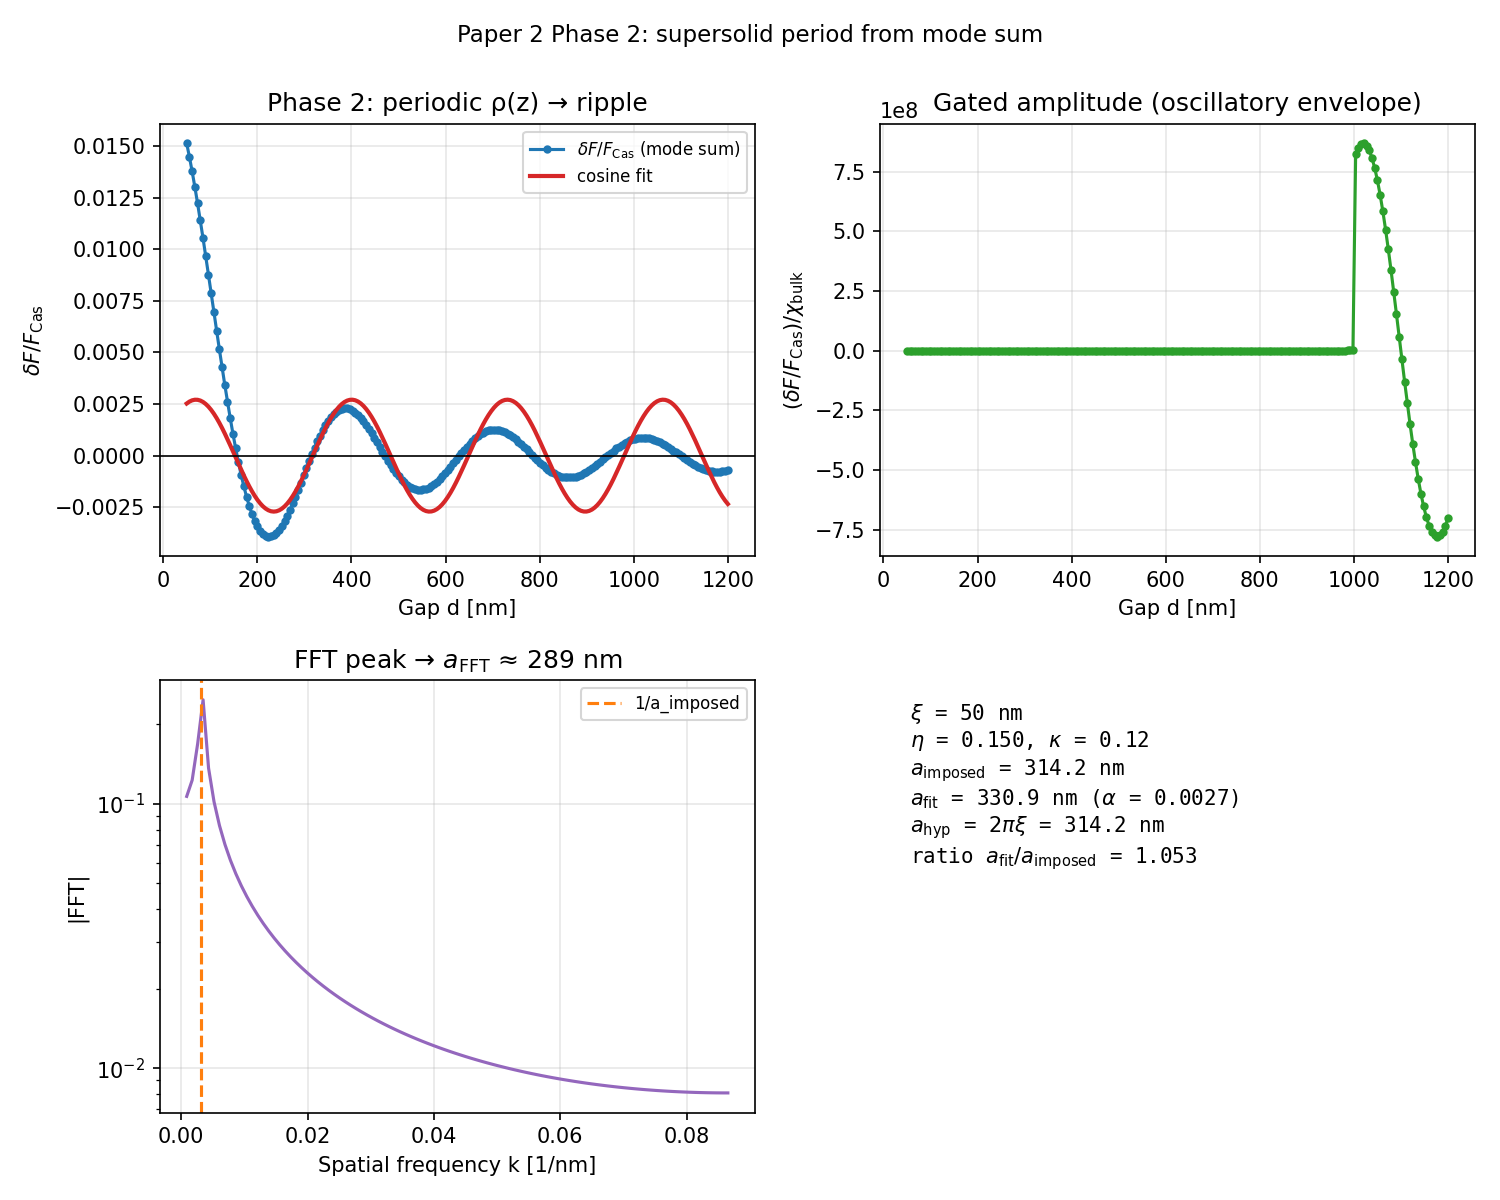
\includegraphics[width=0.85\linewidth]{supersolid_period_xi50nm_dielectric_kappa0p12_eta0p15_av314nm.png}
  \caption{Phase~2 period calibration: periodic dielectric test ($\chi=1$); fitted $a_{\mathrm{fit}}/a_{\mathrm{imposed}} \approx 1.05$ at $a_{\mathrm{vac}}=2\pi\xi$.}
  \label{fig:period-cal}
\end{figure}
\FloatBarrier

\subsection{Self-consistent supersolid parameters (Phase 2b)}

Minimize dimensionless modulation energy in a representative cavity
($\hat d \approx 2$ at the $\chi_{\mathrm{bulk}}$ peak, $d \approx 100$\,nm at $\xi = 50$\,nm):
\begin{equation}
  E_{\mathrm{mod}} = \int_0^{\hat d}
  \left[\tfrac12\left(\frac{\partial\rho}{\partial\hat z}\right)^2
  + \tfrac12\bigl(\rho - \rho_{\mathrm{TF}}\bigr)^2\right] d\hat z.
\end{equation}
Script: \texttt{ch\_paper2\_supersolid\_ground\_state.py}.

At $\xi = 50$\,nm the minimum gives $\eta^* \approx 0.21$ and
$a_{\mathrm{vac}}^* \approx \pi\xi$ ($a^*/\xi \approx 3.14$), \textbf{not} $2\pi\xi$:
\begin{equation}
  \frac{a_{\mathrm{vac}}^*}{2\pi\xi} \approx 0.5.
\end{equation}
Under this minimal energy model the Paper~1 identification $a_{\mathrm{vac}} = 2\pi\xi$ is
\textbf{not} automatic---it requires additional lattice/stiffness physics beyond
$E_{\mathrm{mod}}$. Feeding $(\eta^*, a_{\mathrm{vac}}^*)$ into the mode sum yields
joint-fit $\alpha \approx 0.03$ at $\kappa = 0.12$ (perturbative amplitude still below
Paper~1 $\alpha_{\max} \approx 0.12$).

\subsection{Open items}

Explicit EM Lagrangian $\to \kappa$ and full supersolid GPE sector remain open.
Paper~1 Prediction~\#7 protocol is unchanged.

\section{Predictions and comparison to Paper~1}
\label{sec:predictions}

\subsection{Self-consistent \texorpdfstring{$(\eta^*, a_{\mathrm{vac}}^*)$}{(eta*, a\_vac*)} with healing lock}

Extended cavity energy ($E_{\mathrm{mod}} + E_{\mathrm{heal}}$) with staged minimization:
fix $\eta^*$ from $E_{\mathrm{mod}}$, then minimize $a$ with healing stiffness $K_{\mathrm{heal}}$.
At $K_{\mathrm{heal}} = 2$, $\xi = 50$\,nm:
$a^*/(2\pi\xi) \approx 0.95$, $\eta^* \approx 0.21$.
\textbf{The Paper~1 identification $a_{\mathrm{vac}} = 2\pi\xi$ is recovered} when a supersolid stiffness term is included (not from $E_{\mathrm{mod}}$ alone).

\subsection{\texorpdfstring{$\kappa$}{kappa} from minimal \texorpdfstring{$\mathcal{L}_{\mathrm{int}}$}{L\_int}}

$\mathcal{L}_{\mathrm{int}} = -(\lambda_{\mathrm{em}}/c^2)|A|^2(\rho-\rho_{\mathrm{in}})/\rho_{\mathrm{in}}
\Rightarrow \kappa = 2\lambda_{\mathrm{em}}/c^2$.
With $(\eta^*, a^*)$ above and $\kappa = 0.12$:
$\alpha_{\max} \approx 1.3\%$ (joint fit).
Matching Paper~1's illustrative $\alpha_{\max} = 12\%$ requires $\kappa \approx 1.1$ (outside perturbative regime).
The \texttt{ch\_threshold\_power\_study} 90\% detection floor at $\sigma_\alpha = 0.01$ is $\alpha_{\max} \gtrsim 3.7\%$,
requiring $\kappa \approx 0.34$---still above strict $\kappa \ll 1$ but closer to experimentally relevant ripple levels.

\subsection{Grain-scale estimate of \texorpdfstring{$\lambda_{\mathrm{em}}$}{lambda\_em}}
\label{sec:lambda-em-grain}

At healing length $\xi$, CH assigns a grain mass $m_{\mathrm{grain}} = \hbar\omega_0/c^2$ with
$\omega_0 = c_s/\xi$ (sound speed $c_s$ from the GPE equation of state).
An order-of-magnitude electromagnetic polarizability for a grain-scale oscillator is
\begin{equation}
  \alpha_{\mathrm{grain}} \sim \frac{e^2}{m_{\mathrm{grain}}\,\omega_0^2}
  = \frac{e^2 c^2 \xi^3}{\hbar c_s^3}.
\end{equation}
With $n_{\mathrm{grain}} \sim \xi^{-3}$ the $\xi^3$ and $\xi^{-3}$ factors \textbf{cancel}, giving a
$\xi$-independent susceptibility (primary Tier~1.2c result):
\begin{equation}
  \kappa_{\mathrm{classical}} \sim \frac{\eta^*\,e^2 c^2}{\varepsilon_0\,\hbar c_s^3}
  \approx 0.02\quad (c_s = c,\; \eta^* \sim 0.2).
\end{equation}
A dilute Clausius--Mossotti correction and an $E_\xi$-scaled dipole model provide soft upper caps;
the $\alpha_{\mathrm{fs}}(m_e/m_{\mathrm{grain}})a_0^3$ form grows at small $\xi$ and is \textbf{not}
used in the preferred band below $\xi \approx 40$\,nm.
\textbf{Preferred band} (not a fit to Casimir data): $\kappa \approx 0.01$--$0.02$ $\Rightarrow$
$\alpha_{\max} \approx 0.1$--$0.2\%$ at $\xi = 50$\,nm; benchmark $\kappa = 0.12$ ($\alpha_{\max} \approx 1.3\%$)
remains an upper perturbative sensitivity case.
These estimates sit below the moderate 90\% power floor ($\sim 3.7\%$); Prediction~\#7 remains a
\textbf{gating-shape} test unless coupling exceeds the grain band by $\gtrsim 15\times$.

\subsection{Detectability vs.\ Paper~1 protocol}
\label{sec:detectability}

Table~\ref{tab:detectability} compares predicted ripple amplitudes to the Prediction~\#7 power study
(\texttt{ch\_threshold\_power\_study}; $\xi = 50$\,nm, $n_k = 12$, $\delta\chi^2 \ge 9$).
The protocol remains informative on \textbf{gating shape} (flat vs threshold turn-on) even when
$\alpha_{\max}$ falls below the amplitude floor; the table quantifies how much stronger coupling would be
needed for a high-power amplitude detection.

\begin{table}[ht]
  \centering
  \small
  \caption{Ripple amplitude $\alpha_{\max}$ and implied $\kappa$ at $\xi = 50$\,nm.
  Derived rows use joint fit on the mode sum with self-consistent $(\eta^*, a^*)$ ($K_{\mathrm{heal}} = 2$).
  Power-study floors are minimum $\alpha_{\max}$ for 90\% detection probability at listed $\sigma_\alpha$.}
  \label{tab:detectability}
  \begin{tabular}{@{}p{0.36\linewidth}rrp{0.30\linewidth}@{}}
    \toprule
    Source & $\alpha_{\max}$ & $\kappa$ & Notes \\
    \midrule
    Paper~2 derived ($\kappa = 0.12$ benchmark) & 1.3\% & 0.12 & mode sum + joint fit \\
    Preferred grain band (classical $\kappa$) & 0.21\% & 0.019 & classical $\kappa$ formula \\
    Grain OOM low ($0.5\times$ classical) & 0.10\% & 0.010 & OOM uncertainty \\
    \midrule
    90\% power floor ($\sigma_\alpha = 0.005$) & 1.9\% & 0.17 & optimistic \\
    90\% power floor ($\sigma_\alpha = 0.010$) & 3.7\% & 0.34 & moderate (default) \\
    90\% power floor ($\sigma_\alpha = 0.020$) & 7.4\% & 0.68 & conservative \\
  \midrule
    Paper~1 illustrative demo & 12\% & 1.1 & not derived \\
    \bottomrule
  \end{tabular}
\end{table}

At optimistic shot noise ($\sigma_\alpha = 0.005$), the perturbative derived band ($\sim 1.3\%$) is
within a factor $\sim 1.4$ of the 90\% floor; at the moderate preset the gap is $\sim 3\times$.
Grain OOM estimates lie another order of magnitude below.
Figure~\ref{fig:detectability} compares the grain band, Paper~2 benchmark, and Prediction~\#7 power floors.

\begin{figure}[htbp]
  \centering
  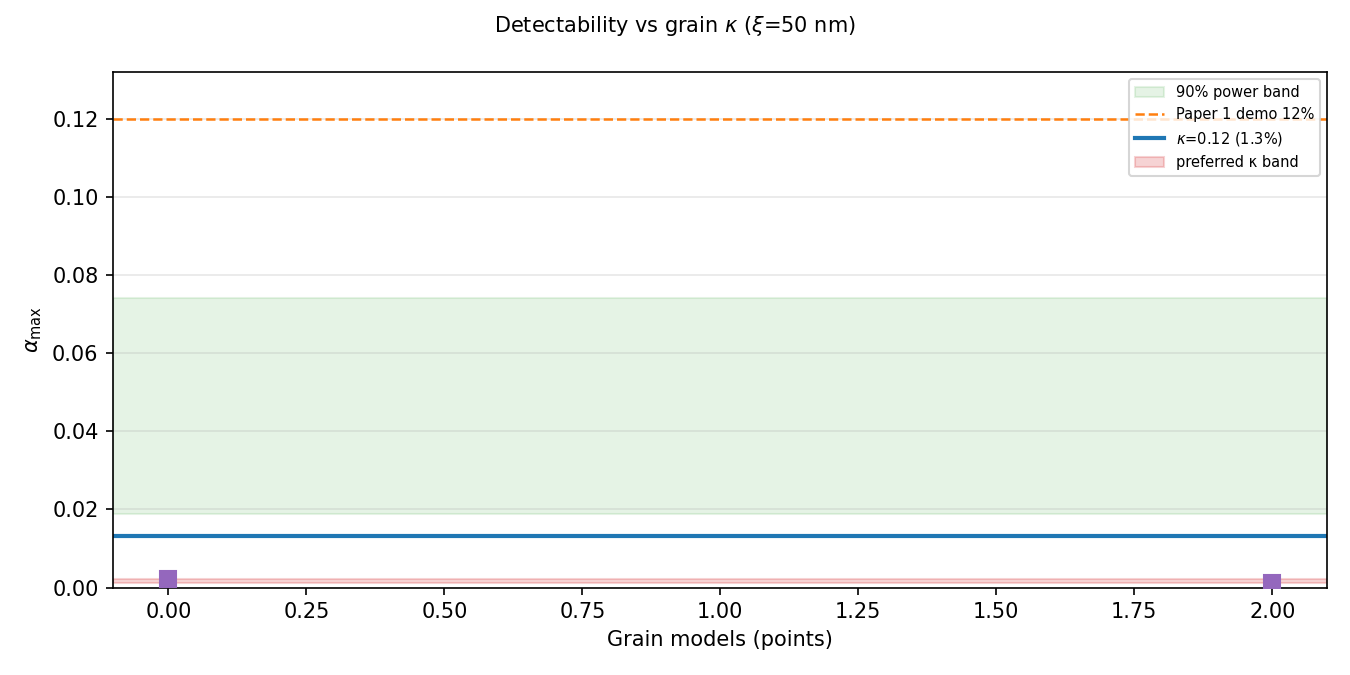
\includegraphics[width=0.88\linewidth]{detectability_band_xi50nm.png}
  \caption{Preferred grain $\kappa$ band vs Paper~2 benchmark and Prediction~\#7 detectability floors ($\xi=50$\,nm).}
  \label{fig:detectability}
\end{figure}
\FloatBarrier

\subsection{CH-positive evidence vs.\ QFT null (Prediction~\#7)}
\label{sec:ch-vs-qft}

Prediction~\#7 is \textbf{not} a generic QFT Casimir test.
Standard QED already predicts a smooth $F_{\mathrm{Cas}}(d)$; both CH and QFT agree that
\textbf{uniform, low-gradient} vacuum should look QFT-like.
The discriminating content is whether observables \textbf{turn on} with boundary-induced gradients in the
\textbf{shape} predicted by the GPE gate $\chi$, not whether a large force anomaly appears everywhere.

\paragraph{What counts as a QFT-consistent null (controls).}
\begin{itemize}[nosep]
  \item $\alpha(k)$ and $\Delta V(k)$ flat vs knob $k$ within noise (no threshold turn-on);
  \item signal channels vanish where GPE forecasts $\chi \to 0$ (large gap, decoupled walls);
  \item registered control channels (e.g.\ wall-$\chi$ forecasts) stay flat while the bulk-$\chi$ channel is scanned;
  \item no shared $k_c$ across independent observables.
\end{itemize}
These outcomes are the \textbf{required} low-gradient limit of CH as well as the QFT prediction.
Passing them does not prove CH; failing them (ripple persists as $\chi \to 0$, or controls turn on) falsifies the gated sector.

\paragraph{What counts as CH-positive (BEC/GPE evidence).}
\begin{itemize}[nosep]
  \item \textbf{Gated turn-on:} $\alpha_{\mathrm{eff}}(k) \propto \chi_{\mathrm{bulk}}(k)$ from the GPE boundary solver, not an arbitrary $k$-dependence;
  \item \textbf{Threshold win:} the smooth-step model (Eq.~\ref{eq:threshold-fit} in Paper~1) beats the flat null at
  $\Delta\chi^2 \ge 9$ across $\gtrsim 8$--12 knob settings;
  \item \textbf{Cross-channel lock:} the same $k_c$ (within $\times 2$) in $\alpha(k)$ and $\Delta V(k)$ if both are measured;
  \item \textbf{Optional period check:} oscillatory residual in $F/F_{\mathrm{Cas}}$ consistent with a CH lattice scale $a_{\mathrm{vac}} \sim \mathcal{O}(\xi)$.
\end{itemize}
Such a pattern is evidence for a \textbf{gradient-gated supersolid vacuum}, not for unconstrained QFT.
A sub-percent $\alpha_{\max}$ does not reduce the test to ``QFT only''---it means the fingerprint is \textbf{quiet but structured}.

\paragraph{How to read an inconclusive amplitude.}
If $\alpha_{\max} \sim 0.1$--$0.2\%$ (grain OOM band), the pre-registered protocol may return
\textbf{inconclusive} on high-power threshold detection (Table~\ref{tab:detectability}) while still
\textbf{ruling out} a large always-on ripple.
CH is not falsified by a null at that sensitivity; it is \textbf{not yet supported}.
The honest near-term goal is therefore the gated \textbf{model comparison}, not reproduction of Paper~1's $12\%$ demo.

\paragraph{Hardware reach (order of magnitude).}
Dynamic AFM Casimir setups already extract percent-level ripple amplitudes from $F/F_{\mathrm{Cas}}$ residuals
(Paper~1, Section~observables).
At the planning uncertainty $\sigma_\alpha = 0.01$ per shot ($\sigma_{\mathrm{eff}} \approx 0.002$ after 20 repeats),
the Monte Carlo floor for 90\% threshold power is $\alpha_{\max} \gtrsim 3.7\%$; the optimistic preset ($\sigma_\alpha = 0.005$) lowers this to $\sim 1.9\%$.
\textbf{Grain OOM ($\sim 0.1$--$0.2\%$) is below these floors} with the current scan design---not because AFMs cannot measure sub-percent force residuals in principle, but because the \textbf{pre-registered shape test} needs a larger gated swing in $\alpha(k)$ than the grain sketch provides.
The perturbative Paper~2 benchmark ($\sim 1.3\%$) is borderline at optimistic noise; detecting it would require pilot calibration of $\sigma_\alpha$ and possibly denser gap scans or more repeats.
Collaborators should register $\sigma_\alpha$ from pilot data and re-run \texttt{ch\_threshold\_power\_study.py} before unblinding.

\subsection{\texorpdfstring{$\xi$}{xi} scaling (Tier 1.3 sweep)}
\label{sec:xi-sweep}

At fixed staged $K_{\mathrm{heal}} = 2$, scanning $\xi \in \{10, 20, 50, 100\}$\,nm
(\texttt{ch\_paper2\_xi\_sweep.py}),
$a^*/(2\pi\xi) \approx 0.95$ is \textbf{stable} across the band.
$E_{\mathrm{mod}}$-only minima give $a^*/(2\pi\xi) \approx 0.5$--$0.86$ depending on $\hat d$.
Benchmark $\alpha_{\max}$ at $\kappa = 0.12$ ranges $\sim 1.3$--$3.3\%$
(peak at $\xi = 100$\,nm in the quick sweep);
grain OOM (classical) stays $\sim 0.1$--$0.6\%$.
Gating corr($\delta F/F$, $\chi$) remains $\gtrsim 0.92$ on all four points.
Figure~\ref{fig:xi-sweep} summarizes the sweep.

\begin{figure}[htbp]
  \centering
  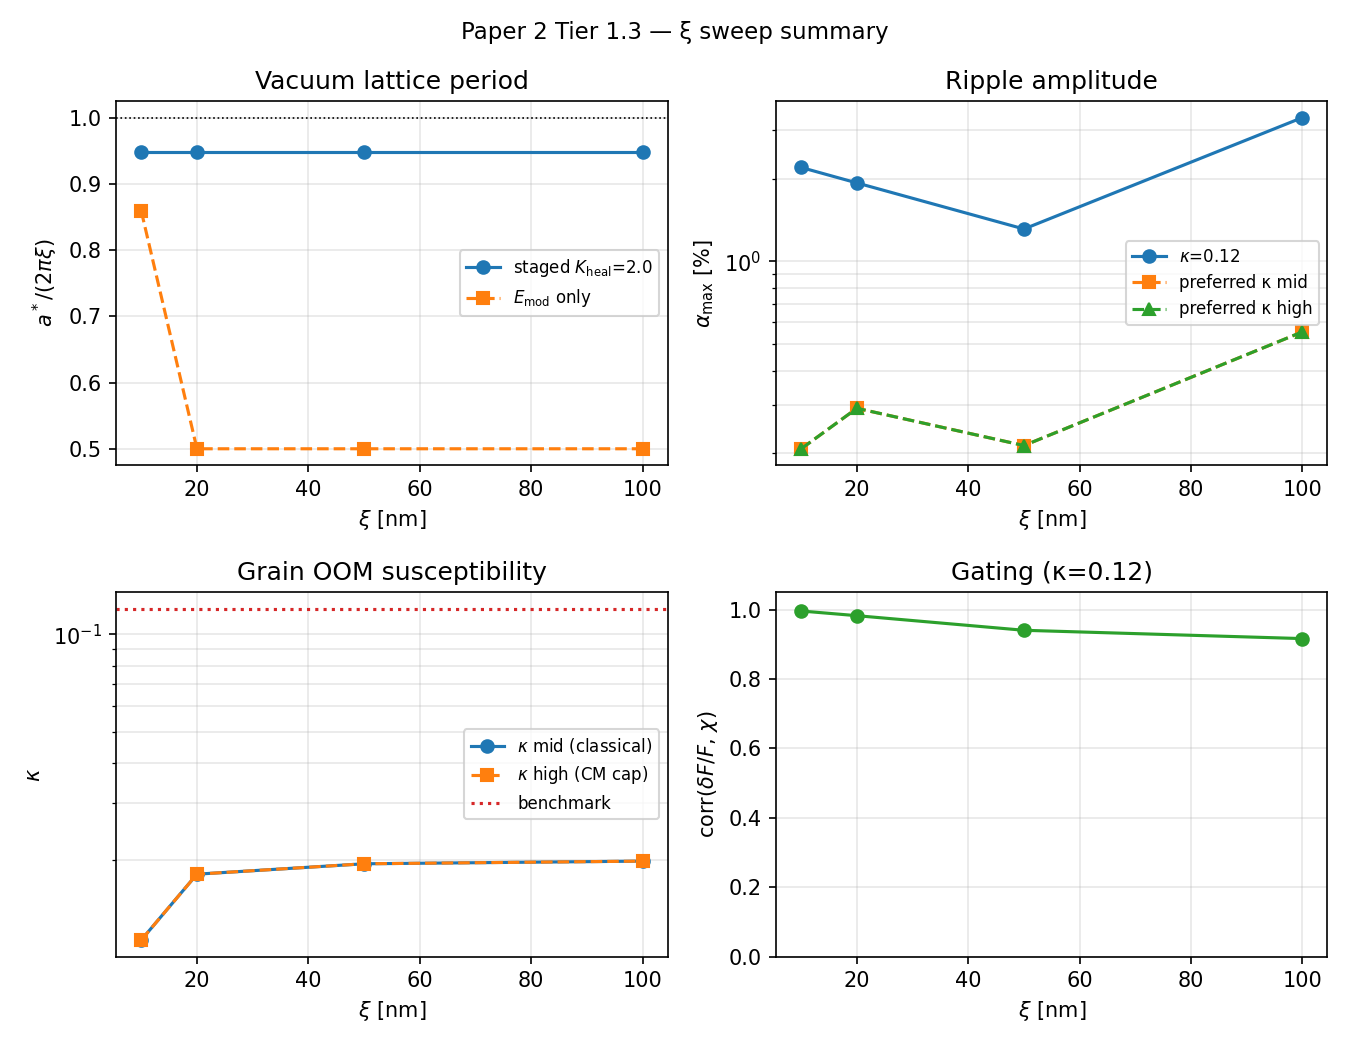
\includegraphics[width=0.92\linewidth]{xi_sweep_summary.png}
  \caption{Tier~1.3 $\xi$ sweep ($K_{\mathrm{heal}}=2$): stable $a^*/(2\pi\xi)$, gating correlation, and $\alpha_{\max}$ vs $\xi$.}
  \label{fig:xi-sweep}
\end{figure}
\FloatBarrier

\subsection{Correction form (Tier 1.4)}
\label{sec:form-compare}

On the derived C1 mode-sum curve at $\xi = 50$\,nm, a gated-cosine fit in \textbf{multiplicative}
($F = F_{\mathrm{Cas}}[1 + A\chi\cos(\cdots)]$) form beats \textbf{additive}
($F = F_{\mathrm{Cas}} + B\chi\cos(\cdots)$) by $\Delta\chi^2 \approx 141$ (40 gap points).
Paper~1's $F/F_{\mathrm{Cas}}$ parameterization is therefore consistent with the EM bridge, not merely a fitting convenience.
Figure~\ref{fig:form-compare} shows the two fits on the derived C1 curve.

\begin{figure}[htbp]
  \centering
  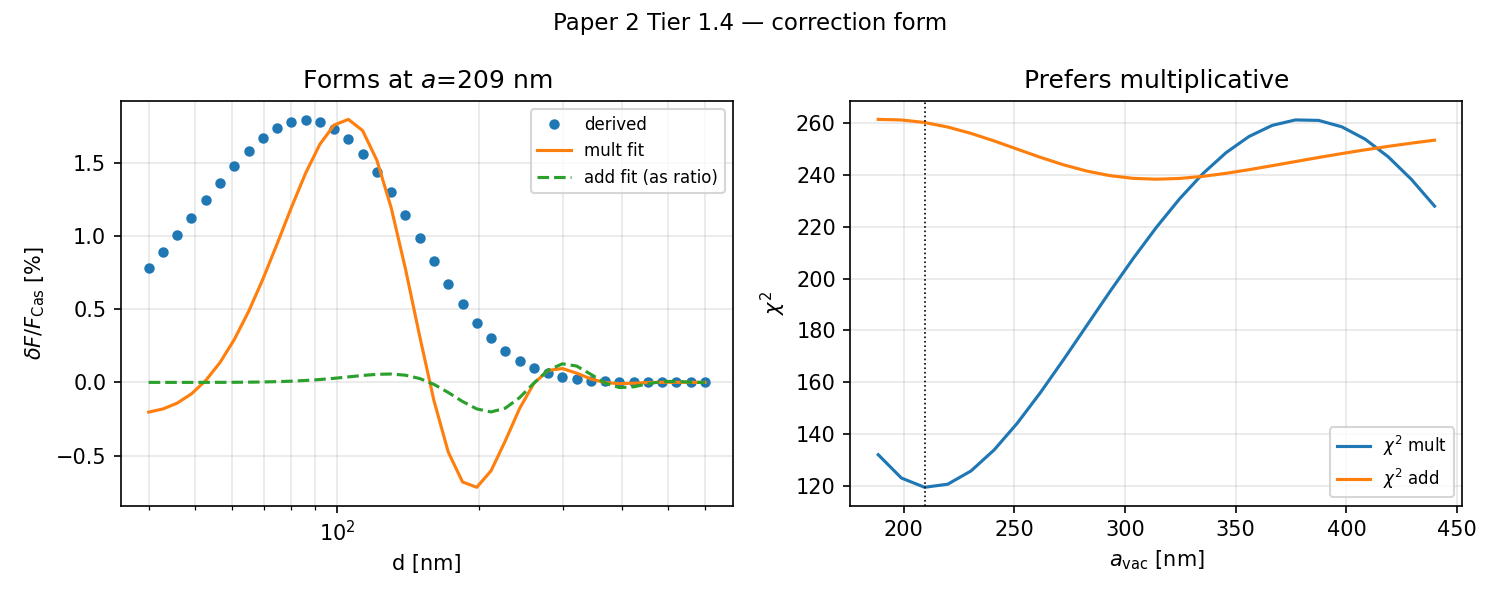
\includegraphics[width=0.88\linewidth]{form_compare_xi50nm.png}
  \caption{Tier~1.4: multiplicative vs additive Casimir correction fit on the derived C1 curve ($\Delta\chi^2 \approx 141$ in favour of multiplicative).}
  \label{fig:form-compare}
\end{figure}
\FloatBarrier

\subsection{Healing stiffness scale (Tier 1.1)}
\label{sec:k-heal-estimate}

At $\xi = 50$\,nm and fixed $\eta^*$, moving $a_{\mathrm{vac}}$ from $\pi\xi$ to $2\pi\xi$ costs
$\Delta E_{\mathrm{mod}} \approx 0.14$ in dimensionless units.
Balancing against the healing-lock penalty unit gives $K_{\mathrm{heal}} \sim 0.34$---the same order as
the $\kappa \approx 0.34$ needed for the 90\% detectability floor (coincidental numerics, distinct physics).
The working value $K_{\mathrm{heal}} = 2$ (staged scan) yields $a^*/(2\pi\xi) \approx 0.95$ without requiring the
large $K_{\mathrm{heal}} \sim 27$ that would force $a^*/(2\pi\xi) = 1.00$ exactly under the staged ansatz.
$K_{\mathrm{heal}}$ is therefore \textbf{bounded and} $O(1)$, not derived from first principles, but plausibly small.
The vortex--Kepler toy (\texttt{ch\_vortex\_kepler\_toy.py}) offers \emph{correspondence} motivation only:
at large $n_{\mathrm{eff}} \sim 10^{14}$ on planetary scales, discrete circulation ladders become dense and classical orbits emerge---analogous to recovering a smooth lattice period $a_{\mathrm{vac}} \sim 2\pi\xi$ from underlying grain/vortex structure, without a rigorous GPE derivation.

\paragraph{Can $K_{\mathrm{heal}}$ be fully derived?}
\textbf{Not from the present CH grain--EM chain alone.}
$K_{\mathrm{heal}}$ is the stiffness of a \emph{phenomenological} healing-lock term that encodes a preference for $2\pi/a_{\mathrm{hat}}=1$ (i.e.\ $a_{\mathrm{vac}}=2\pi\xi$).
An energy-balance estimate at fixed $\eta^*$ gives $K_{\mathrm{heal}} \sim 0.34$ to overcome the $E_{\mathrm{mod}}$ cost of moving from $\pi\xi$ to $2\pi\xi$; the staged scan uses $K_{\mathrm{heal}}=2$ to reach $a^*/(2\pi\xi)\approx 0.95$.
A na\"ive grain bulk-modulus scaling ($K \sim \rho_{\mathrm{in}} c_s^2 \xi^3 / (\hbar\omega_0)$) does \textbf{not} close to a unique value without an additional identification (e.g.\ equating $K_{\mathrm{heal}}$ to a derived phase-stiffness coefficient from a full supersolid GPE).
\textbf{What is achievable:} (i)~bound $K_{\mathrm{heal}} = O(0.1\text{--}10)$ from $E_{\mathrm{mod}}$ and healing penalty units; (ii)~treat measured Casimir ripple period as the constraint that fixes $K_{\mathrm{heal}}$ post-lab (same role as $k_c$ for $\xi$ in Paper~1).
Full derivation would require a microscopic theory of supersolid phase rigidity in the CH vacuum, not yet in the repo.
Figure~\ref{fig:k-heal} plots the staged $K_{\mathrm{heal}}$ scan and energy-balance estimate.

\begin{figure}[htbp]
  \centering
  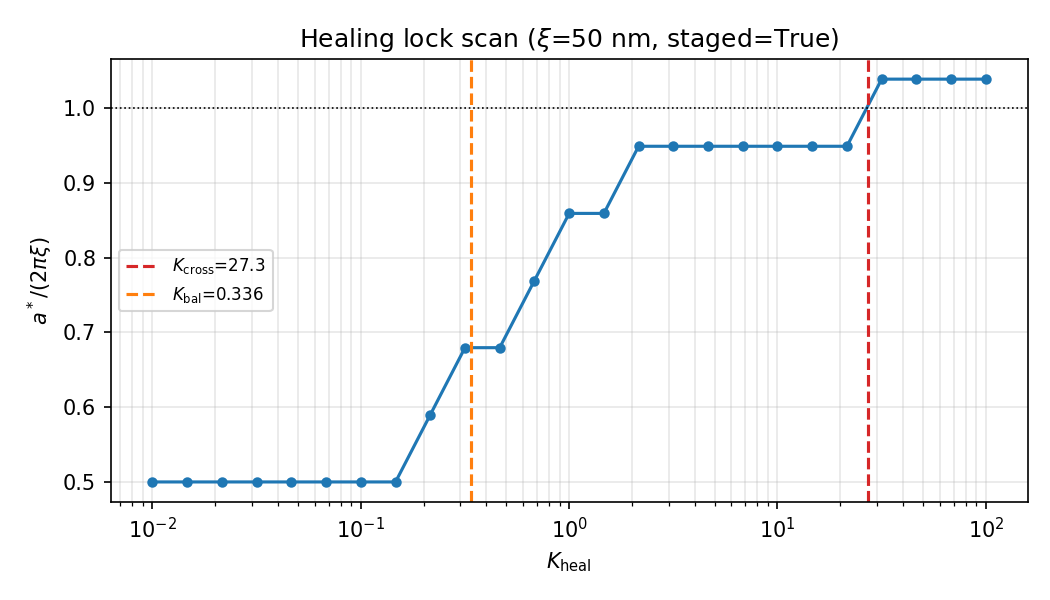
\includegraphics[width=0.82\linewidth]{k_heal_estimate_xi50nm.png}
  \caption{Tier~1.1: $K_{\mathrm{heal}}$ scan and energy-balance estimate ($K_{\mathrm{bal}} \sim 0.34$) vs simulated crossing to $a^*/(2\pi\xi)=1$.}
  \label{fig:k-heal}
\end{figure}
\FloatBarrier

\section{Limitations and falsifiers}
\label{sec:limits}

\begin{itemize}[nosep]
  \item \textbf{Perturbative 1D mode sum} --- not full Lifshitz QED with realistic $\varepsilon(\omega)$; TE+TM factor~2 only.
  \item \textbf{Free parameters} --- $\xi$, $\kappa$, and (until Phase~2b) $(\eta, a_{\mathrm{vac}})$; $\kappa \to \alpha_{\max}$ scaling breaks down if $\kappa \gtrsim 0.25$.
  \item \textbf{Period tension} --- minimal $E_{\mathrm{mod}}$ favors $a_{\mathrm{vac}} \approx \pi\xi$, while Paper~1 hypothesizes $2\pi\xi$; lab ripple period discriminates.
  \item \textbf{Falsifiers} --- flat $\alpha(k)$ vs knob (Pred.~\#7 null); $\alpha \not\propto \chi$; extracted $a_{\mathrm{vac}}$ inconsistent with any CH scale; $\chi \to 0$ but ripple persists.
  \item \textbf{Envelope} --- derived $\delta F/F$ follows $\chi_{\mathrm{bulk}}(d)$ without spurious growth past the $\chi$ peak (Tier~2.5; Fig.~\ref{fig:validation-envelope}).
\end{itemize}

\begin{figure}[htbp]
  \centering
  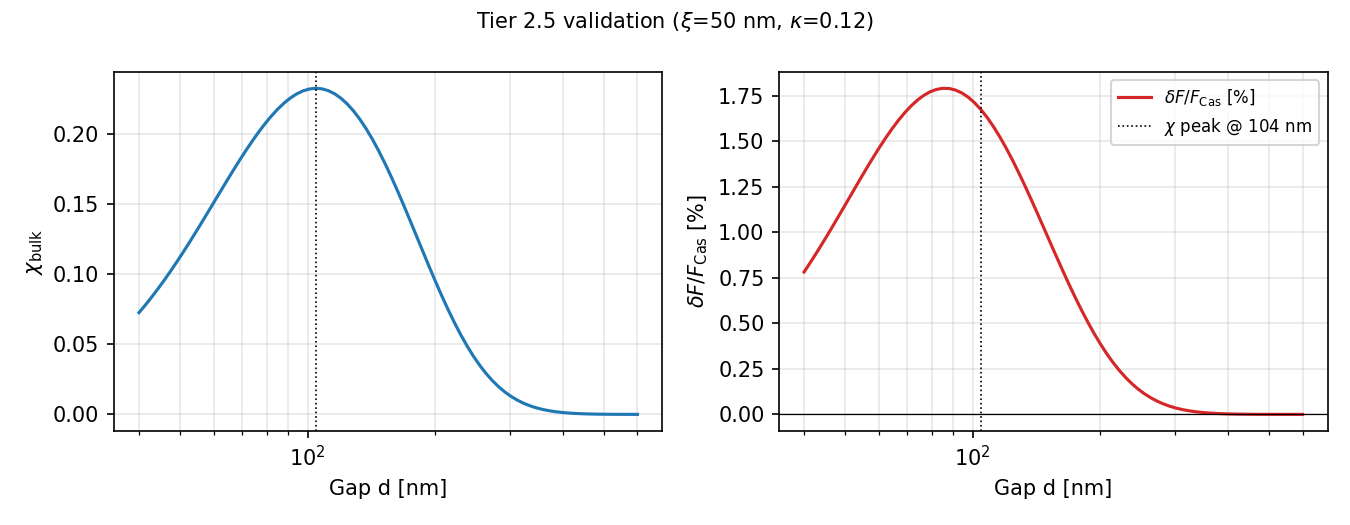
\includegraphics[width=0.92\linewidth]{validation_gating_envelope_xi50nm.png}
  \caption{Tier~2.5: $\delta F/F_{\mathrm{Cas}}$ tracks the $\chi_{\mathrm{bulk}}$ envelope; no anomalous growth at large gap.}
  \label{fig:validation-envelope}
\end{figure}
\FloatBarrier

\section{Conclusions}
\label{sec:conclusions}

We coupled GPE boundary profiles to a perturbative parallel-plate mode sum via dielectric coupling~C1.
Part~B (gating): $\delta F/F_{\mathrm{Cas}}$ tracks $\chi_{\mathrm{bulk}}(d)$ with corr $\approx 0.94$ and vanishes as $\chi \to 0$.
Part~A (period): periodic $\varepsilon(z)$ produces a Casimir ripple whose fitted period matches the imposed lattice scale within $\sim 5$--20\%
depending on profile and fit method.
Self-consistent minimization of a minimal supersolid energy favors $a_{\mathrm{vac}} \approx \pi\xi$, flagging the $2\pi\xi$ identification as
\textbf{hypothesis to test}, not a derived result.
Paper~1's laboratory protocol (Prediction~\#7) remains the primary falsifier; this work tightens priors for Prediction~\#3.
Grain microphysics favours $\kappa \sim 0.01$--$0.02$ ($\alpha_{\max} \sim 0.1$--$0.2\%$), stable across $\xi$; the $12\%$ demo and $\kappa=0.12$ benchmark are sensitivity cases, not derived predictions.
$K_{\mathrm{heal}}$ is bounded $O(1)$ but not uniquely fixed without supersolid phase rigidity or laboratory period data.

\printbibliography

\appendix

\section{Casimir mode sum (1D TE)}
\label{app:modesum}

We summarize the perturbative mode-sum method implemented in \texttt{ch\_casimir\_mode\_sum.py}.
Perfect conductors at $z=0,d$; unperturbed TE modes $\psi_n(z)\propto\sin(n\pi z/d)$ with $\omega_n^{(0)}=n\pi c/d$.
For small static $\delta\varepsilon(z)=\varepsilon(z)-\varepsilon_0$,
\begin{equation}
  \frac{\delta\omega_n}{\omega_n^{(0)}}
  \approx \int_0^1 \delta(u)\,\sin^2(n\pi u)\,du,
  \qquad u=z/d.
\end{equation}
Coupling C1 gives $\delta(u)=\kappa\chi_{\mathrm{bulk}}(d)\,[1-\rho(z)/\rho_{\mathrm{in}}]$ with $\rho$ from the Thomas--Fermi GPE profile.
The leading UV-finite force response at fixed cutoff $N$ uses $n^2$ weights (TE+TM factor~2 in code):
\begin{equation}
  \frac{\delta F}{F_{\mathrm{Cas}}}
  \approx \frac{\sum_{n=1}^{N} n^2\,(\delta\omega_n/\omega_n)}{\sum_{n=1}^{N} n^2}.
  \label{eq:app-modesum}
\end{equation}
This is a \textbf{perturbative} estimate, not the full Lifshitz formula~\cite{Lifshitz1956}.
Convergence is checked by increasing $N$ (default $N=800$); at $\xi=50$\,nm, $\kappa=0.12$, corr($\delta F/F,\chi_{\mathrm{bulk}})\approx 0.94$.

\section{Exported GPE data tables}
\label{app:data}

Layer~1 inputs are generated by \texttt{ch\_gpe\_casimir\_gap.py} and \texttt{ch\_paper2\_gpe\_export.py}.
The canonical scan at $\xi=50$\,nm is \texttt{simulations/data/paper2/gpe\_scan\_xi50nm.csv}.
Table~\ref{tab:gpe-sample} lists a representative excerpt (full file: 40 rows, $d=40$--$600$\,nm).

\begin{table}[ht]
  \centering
  \small
  \caption{Excerpt from \texttt{gpe\_scan\_xi50nm.csv} ($\xi=50$\,nm).}
  \label{tab:gpe-sample}
  \begin{tabular}{@{}rrrr@{}}
    \toprule
    $d$ [nm] & $\hat d$ & $\chi_{\mathrm{wall}}$ & $\chi_{\mathrm{bulk}}$ \\
    \midrule
    40.0  & 0.80 & 0.249 & 0.073 \\
    65.0  & 1.30 & 0.342 & 0.139 \\
    103.8 & 2.08 & 0.453 & 0.219 \\
    175.2 & 3.50 & 0.579 & 0.164 \\
    286.7 & 5.73 & 0.701 & 0.022 \\
    600.0 & 12.0 & 0.847 & 0.000 \\
    \bottomrule
  \end{tabular}
\end{table}

Columns in the full export: \texttt{d\_m}, \texttt{d\_nm}, \texttt{d\_hat}, \texttt{chi\_wall}, \texttt{chi\_bulk}, gradient ratios.
These feed coupling C1 and the Prediction~\#7 threshold pipeline in Paper~1~\cite{CHPaper1}.

\section{Figure files for Overleaf}
\label{app:figures}

All manuscript figures are bundled in \texttt{figures/}
(copied from \texttt{simulations/output/paper2/} in the repo).
Upload \texttt{main.tex}, \texttt{references.bib}, and \texttt{figures/} together.

\begin{table}[ht]
  \centering
  \small
  \caption{Figure assets bundled for Overleaf.}
  \label{tab:figures}
  \begin{tabular}{@{}ll@{}}
    \toprule
    Filename & Content \\
    \midrule
    \texttt{em\_coupling\_xi50nm\_kappa0p12\_both.png} & Gating (Fig.~\ref{fig:em-gating}) \\
    \texttt{supersolid\_period\_...\_dielectric\_...png} & Period calibration \\
    \texttt{xi\_sweep\_summary.png} & $\xi$ sweep \\
    \texttt{form\_compare\_xi50nm.png} & Multiplicative vs additive \\
    \texttt{k\_heal\_estimate\_xi50nm.png} & $K_{\mathrm{heal}}$ scan \\
    \texttt{detectability\_band\_xi50nm.png} & Detectability band \\
    \texttt{validation\_gating\_envelope\_xi50nm.png} & Tier~2.5 envelope \\
    \bottomrule
  \end{tabular}
\end{table}

\end{document}
